%! TEX program = <xelatex>

\documentclass{beamer}
\usepackage[utf8]{inputenc}
\usepackage[T1]{fontenc}
\usepackage{caption}
\usepackage{booktabs}

\usetheme{itasca}

\captionsetup[figure]{slc=off}

\title{The Itasca Beamer Theme}
\subtitle{Information without Distractions}
\date[2014-10-30]{October 30, 2014}
\author[P. M. Schnell]{Patrick M. Schnell}

\begin{document}

\begin{frame}
	\titlepage
\end{frame}

\begin{frame}
	\frametitle{Outline}
	\tableofcontents
\end{frame}

\section{Introduction}

\sectionpage

\begin{frame}{Background}

	\textbf{Itasca State Park} in northern Minnesota contains the headwaters of the Mississippi River.

	\begin{figure}\label{fig:itasca}
	\centering
	\captionbox
		{``Mississippi River at Itasca'' by Mark Evans from Orange City, USA - MN18. Licensed under Creative Commons Attribution 2.0 via Wikimedia Commons - \href{http://commons.wikimedia.org/wiki/File:Mississippi_River_at_Itasca.jpg}{Source}}
		{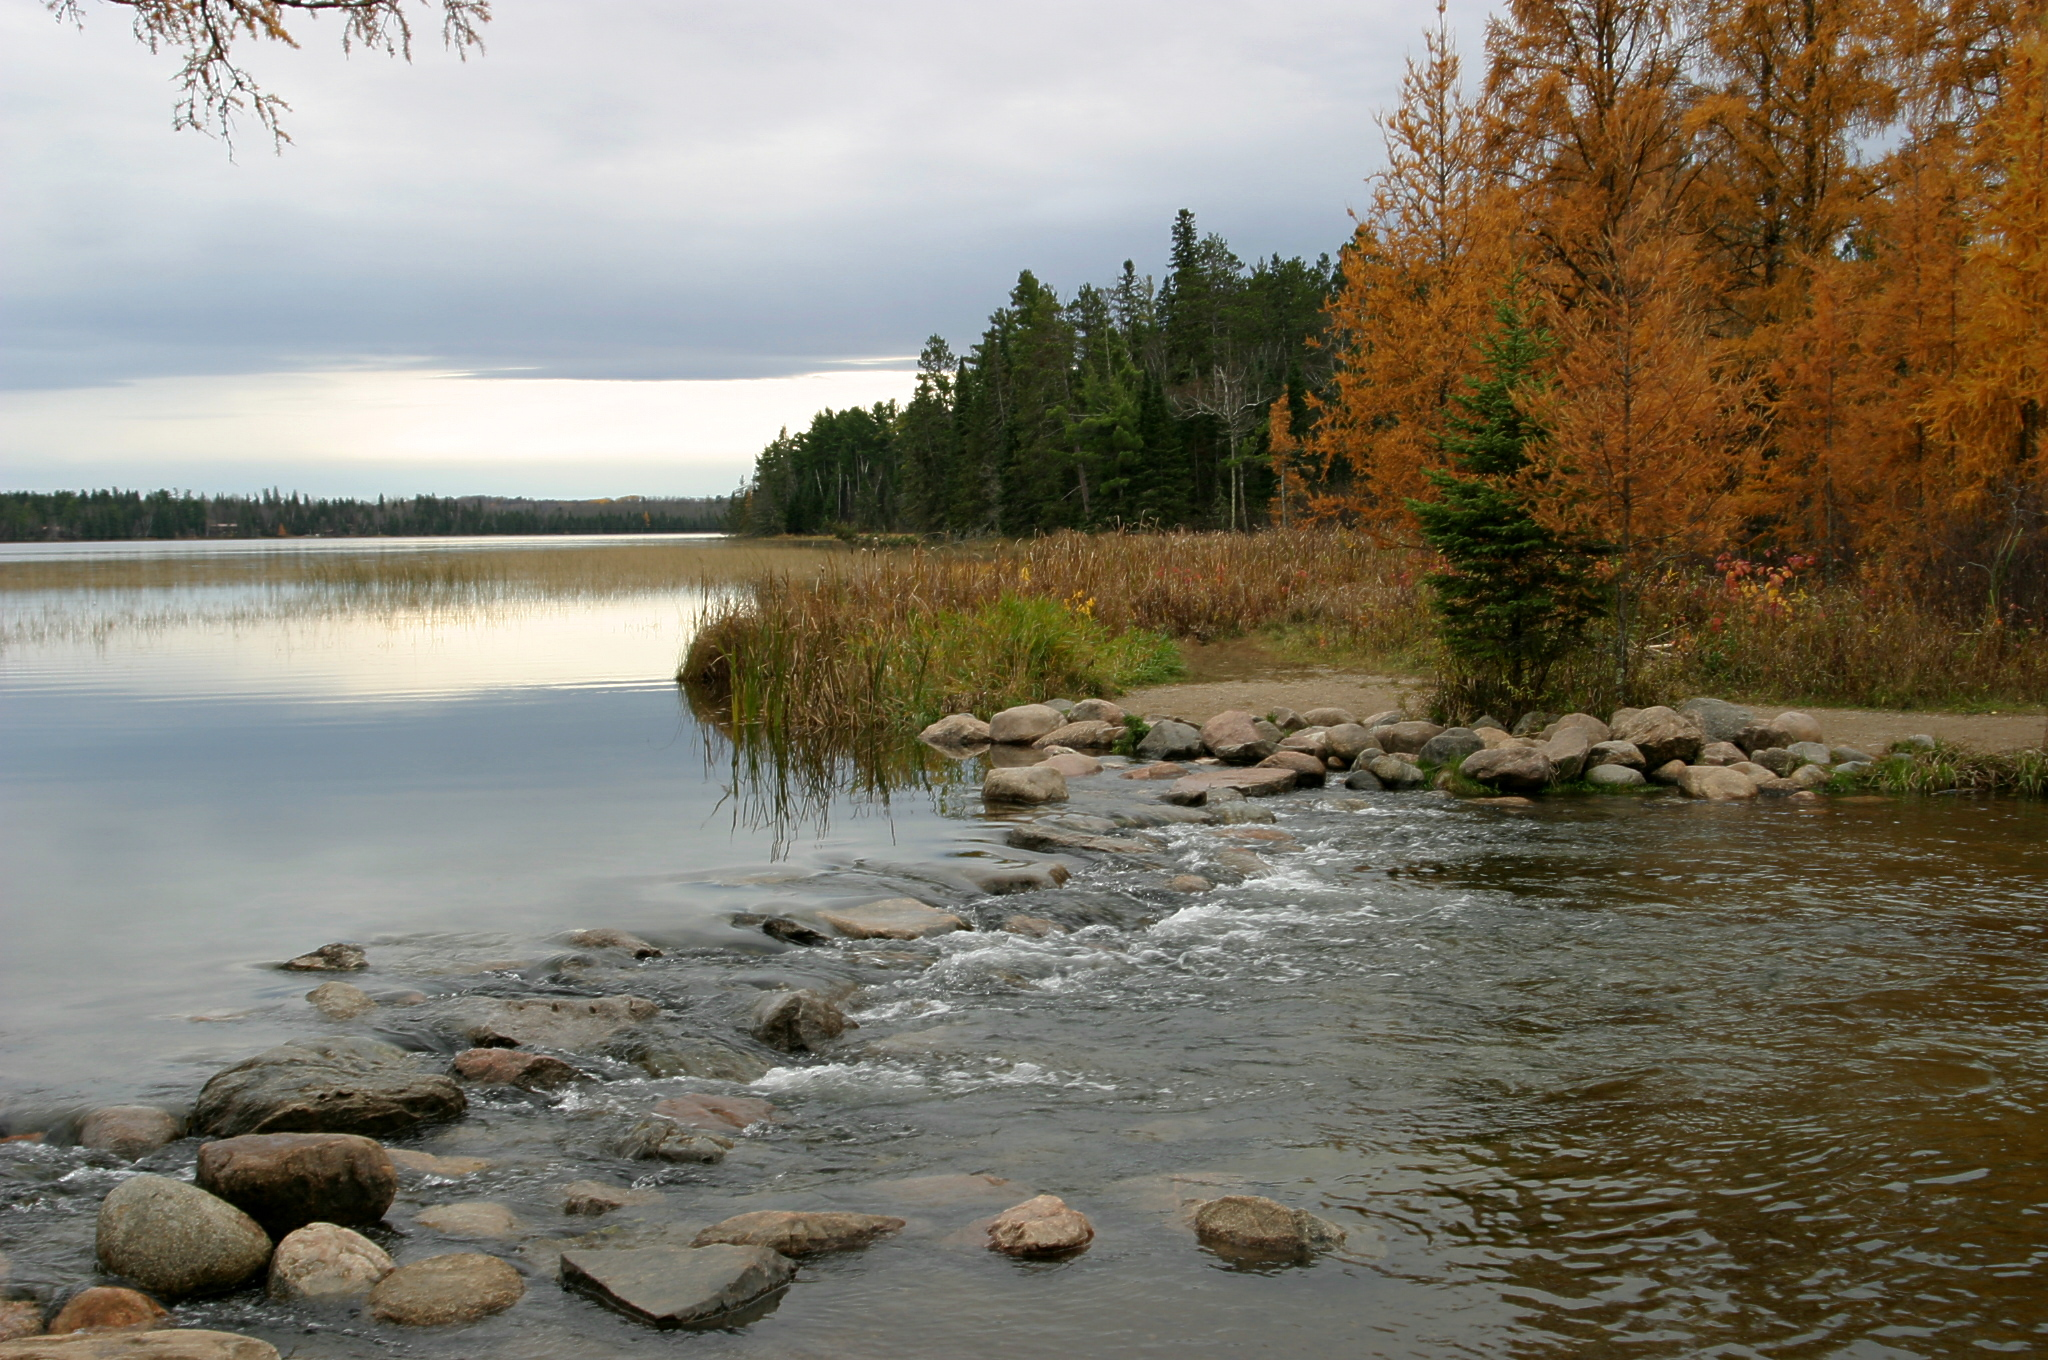
\includegraphics[trim=0cm 4cm 0cm 4cm, clip, width=\textwidth]{graphics/mississippi-river}}
	\end{figure}
\end{frame}

\begin{frame}{Requirements}
	\begin{itemize}
		\item \texttt{XeLaTeX} build program
		\item Fira Sans and Fira Mono fonts
	\end{itemize}
\end{frame}

\begin{frame}{Goals}
	\begin{itemize}
		\item Easy to focus on inner frame
		\item Informative but unobtrusive outer frame
		\item Proper emphasis on important elements
		\item Math, table, and figure support
		\item Aesthetically pleasing
	\end{itemize}
\end{frame}

\section{Colors and Fonts}

\sectionpage

\begin{frame}{Foreground Colors}
	\begin{itemize}
		\item \textbf{Dark gray text} is muted but easy on the eyes
		\item \textbf{Blue secondary color} is consistent and highlights without clashing
		\item \textbf{Dark red \alert{alert} color} emphasizes in line without distracting from the rest of the frame
	\end{itemize}
\end{frame}

\begin{frame}{Background Colors}
	\begin{itemize}
		\item \textbf{Off-white background} reduces eye strain while maintaining clear appearance
		\item \textbf{Light text color} in header and footer is readable but does not draw attention
	\end{itemize}
\end{frame}

\begin{frame}{Fonts}
	\begin{itemize}
		\item \textbf{Fira Sans} primary font is readable and modern
		\item \texttt{Fira Mono} monospaced font is consistent with primary font
	\end{itemize}
\end{frame}

\section{Outer Theme}

\sectionpage

\begin{frame}{Header}
	\begin{itemize}
		\item \textbf{Section titles} anchor slides in context
		\item \textbf{Bookmarks} allow quick navigation between sections
		\item \textbf{Dividing line} separates navigation from inner frame
	\end{itemize}
\end{frame}

\begin{frame}{Footer}
	\begin{itemize}
		\item \textbf{Page number} allows easy referencing of slides
		\item \textbf{No total number} of pages to distract the audience
		\item \textbf{No navigation bar} cluttering slide with redundant features
	\end{itemize}
\end{frame}

\section{Inner Theme}

\begin{frame}{Enumerate and Itemize}
	\begin{itemize}
		\item Nested lists
			\begin{enumerate}
				\item First item
				\item Second item
			\end{enumerate}
		\item
			Sensible spacing and indentation
	\end{itemize}
\end{frame}

\begin{frame}{Display Equations}
	Readable equations are consistent with primary text.
	\begin{equation*}
		\sum_{n = 0}^{\infty} \frac{x^n}{n!} = e^{x}
	\end{equation*}
\end{frame}

\begin{frame}{Theorems}
	\begin{definition}[Prime Number]
		A number $n \in \mathbb{N}$ is prime if its only divisors are $1$ and $n$.
	\end{definition}

	\begin{theorem}[Euclid]
		There are infinitely many prime numbers.
	\end{theorem}

	\begin{proof}
		Left as an exercise for the reader.
	\end{proof}

\end{frame}

\begin{frame}{Tables}
	\begin{table}
		\begin{tabular}{ccc}
		\toprule
		Experiment & Mean & Standard Error \\
		\midrule
		January & 10 & 1 \\
		February & 20 & 2 \\
		March & 30 & 5 \\
		\bottomrule
		\end{tabular}

		\caption{Numerals are set in monospace font.}
	\end{table}
\end{frame}

\section{Conclusion}

\sectionpage

\begin{frame}{Licensing}
\textbf{Copyright (c) 2014 Patrick Schnell}

The Itasca Beamer theme is provided under the MIT License, and may be used, modified, or reproduced as long as the copyright notice is included in all copies and substantial portions of the theme.
There are no restrictions on presentations produced using this theme.
\end{frame}

\end{document}